\documentclass[12pt,dvipdfmx]{beamer}
\usepackage{graphicx}
\DeclareGraphicsExtensions{.pdf}
\DeclareGraphicsExtensions{.eps}
\graphicspath{{out/}{out/tex/}{out/pdf/}{out/eps/}{out/tex/gpl/}{out/tex/svg/}{out/pdf/dot/}{out/pdf/gpl/}{out/pdf/img/}{out/pdf/odg/}{out/pdf/svg/}{out/eps/dot/}{out/eps/gpl/}{out/eps/img/}{out/eps/odg/}{out/eps/svg/}}
\usepackage{listings, jlisting}
\usepackage{fancybox}
\usepackage{fancyvrb}
\usepackage{hyperref}
\usepackage{comment}
\usepackage{color}
\usepackage{subfigure}
\usepackage[font=footnotesize]{caption}
% 図表番号を振る
\setbeamertemplate{caption}[numbered]
% 下の図表番号のスペースを除去
\setlength\abovecaptionskip{0.5em}

\newenvironment{wideitemize}{\itemize\setlength{\itemsep}{1em}}{\enditemize}
\newenvironment{wideitemize2}{\itemize\setlength{\itemsep}{0.2em}}{\enditemize}
\newenvironment{widedescription}{\description\setlength{\itemsep}{1em}}{\enddescription}
\newenvironment{widedescription2}{\description\setlength{\itemsep}{0.2em}}{\enddescription}

%%%%%%%%%%%%%%%%%%%%%%%%%%%
%%% themes
%%%%%%%%%%%%%%%%%%%%%%%%%%%
\usetheme{Madrid}
%% no navigation bar
% default boxes Bergen Boadilla Madrid Pittsburgh Rochester
%% tree-like navigation bar
% Antibes JuanLesPins Montpellier
%% toc sidebar
% Berkeley PaloAlto Goettingen Marburg Hannover Berlin Ilmenau Dresden Darmstadt Frankfurt Singapore Szeged
%% Section and Subsection Tables
% Copenhagen Luebeck Malmoe Warsaw

%%%%%%%%%%%%%%%%%%%%%%%%%%%
%%% innerthemes
%%%%%%%%%%%%%%%%%%%%%%%%%%%
% \useinnertheme{circles}	% default circles rectangles rounded inmargin

%%%%%%%%%%%%%%%%%%%%%%%%%%%
%%% outerthemes
%%%%%%%%%%%%%%%%%%%%%%%%%%%
% outertheme
% \useoutertheme{default}	% default infolines miniframes smoothbars sidebar sprit shadow tree smoothtree


%%%%%%%%%%%%%%%%%%%%%%%%%%%
%%% colorthemes
%%%%%%%%%%%%%%%%%%%%%%%%%%%
\usecolortheme{seahorse}
%% special purpose
% default structure sidebartab 
%% complete 
% albatross beetle crane dove fly seagull 
%% inner
% lily orchid rose
%% outer
% whale seahorse dolphin

%%%%%%%%%%%%%%%%%%%%%%%%%%%
%%% fontthemes
%%%%%%%%%%%%%%%%%%%%%%%%%%%
\usefonttheme{serif}  
% default professionalfonts serif structurebold structureitalicserif structuresmallcapsserif

%%%%%%%%%%%%%%%%%%%%%%%%%%%
%%% generally useful beamer settings
%%%%%%%%%%%%%%%%%%%%%%%%%%%
% 
\AtBeginDvi{\special{pdf:tounicode EUC-UCS2}}
% do not show navigation
\setbeamertemplate{navigation symbols}{}
% show page numbers
\setbeamertemplate{footline}[frame number]

%%%%%%%%%%%%%%%%%%%%%%%%%%%
%%% define some colors for convenience
%%%%%%%%%%%%%%%%%%%%%%%%%%%

\newcommand{\mido}[1]{{\color{green}#1}}
\newcommand{\mura}[1]{{\color{purple}#1}}
\newcommand{\ore}[1]{{\color{orange}#1}}
\newcommand{\ao}[1]{{\color{blue}#1}}
\newcommand{\aka}[1]{{\color{red}#1}}

\setbeamercolor{ex}{bg=cyan!20!white}

%%%%%%%%%%%%%%%%%%%%%%%%%%%
%%% how to typset code
%%%%%%%%%%%%%%%%%%%%%%%%%%%

\lstset{language=C++,
    basicstyle=\ttfamily\scriptsize,
    keywordstyle=\color{blue}\ttfamily,
    stringstyle=\color[cmyk]{0,0.6,1,0.2}\ttfamily,
    commentstyle=\color[cmyk]{1,0.4,1,0}\ttfamily,
    identifierstyle=\color[cmyk]{0,1,0.1,0.8}\ttfamily,
    morecomment=[l][\color{magenta}]{\#},
    breaklines = true,
    escapechar=\@,
}

% \lstset{language = C,
% numbers = left,
% numberstyle = {\tiny \emph},
% numbersep = 10pt,
% breaklines = true,
% breakindent = 40pt,
% frame = tlRB,
% frameround = ffft,
% framesep = 3pt,
% rulesep = 1pt,
% rulecolor = {\color{blue}},
% rulesepcolor = {\color{blue}},
% flexiblecolumns = true,
% keepspaces = true,
% basicstyle = \ttfamily\scriptsize,
% identifierstyle = ,
% commentstyle = ,
% stringstyle = ,
% showstringspaces = false,
% tabsize = 4,
% escapechar=\@,
% }


\title{数学・物理をプログラミングで考える}
\institute{}
\author{水2: 田浦健次朗 \\
TA 高品剛大 (修士2年) 松岡きしん (修士1年) \\
%火4: 山崎俊彦 \\
%TA 中村 遵介 (修士1年) Yiwei Zhang (修士1年) \\
}

\date{}

\AtBeginSubsection[] % Do nothing for \section*
{
\begin{frame}
\frametitle{Contents}
\tableofcontents[currentsection,currentsubsection]
\end{frame}
}

\begin{document}
\maketitle

%%%%%%%%%%%%%%%%% 
\begin{frame}
  \frametitle{計算が支える科学, 工学, AI, \ldots の例}
  \begin{itemize}
  \item 創薬, 医学, 材料 (分子, 量子力学)

    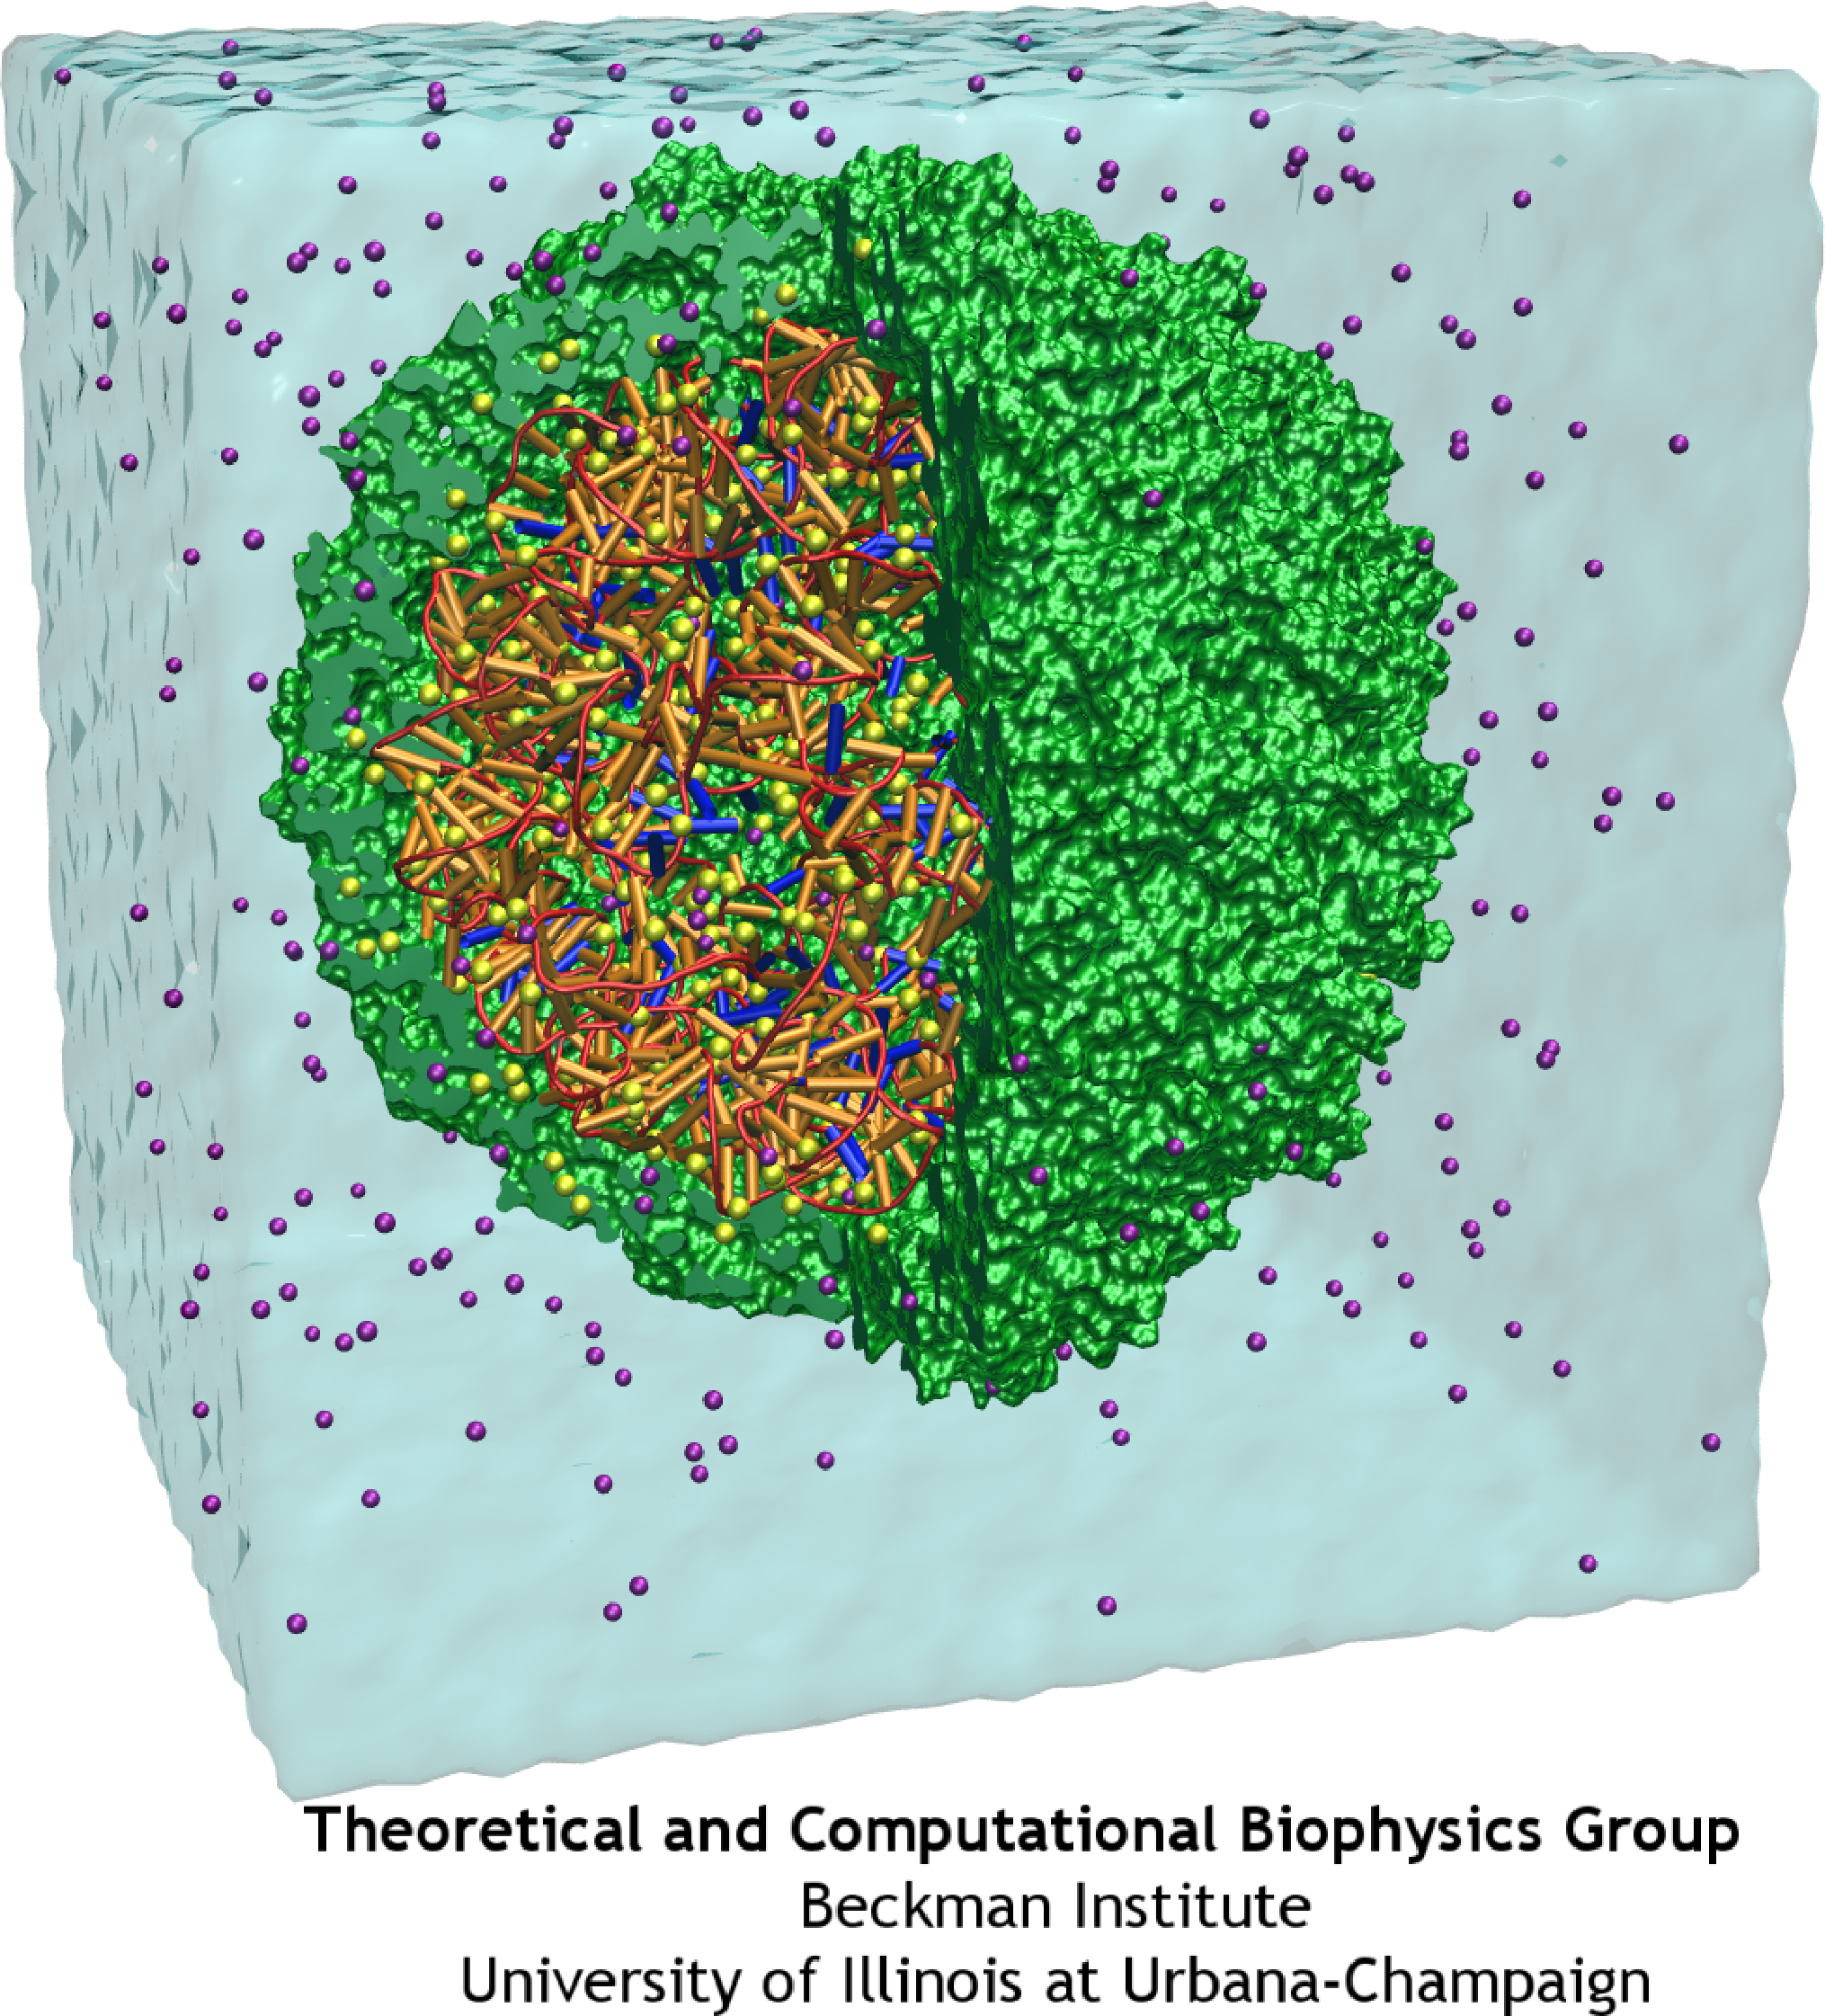
\includegraphics[width=0.25\textwidth]{out/pdf/img/virus.pdf}
    {\tiny\url{http://www.ks.uiuc.edu/Research/STMV/}}

    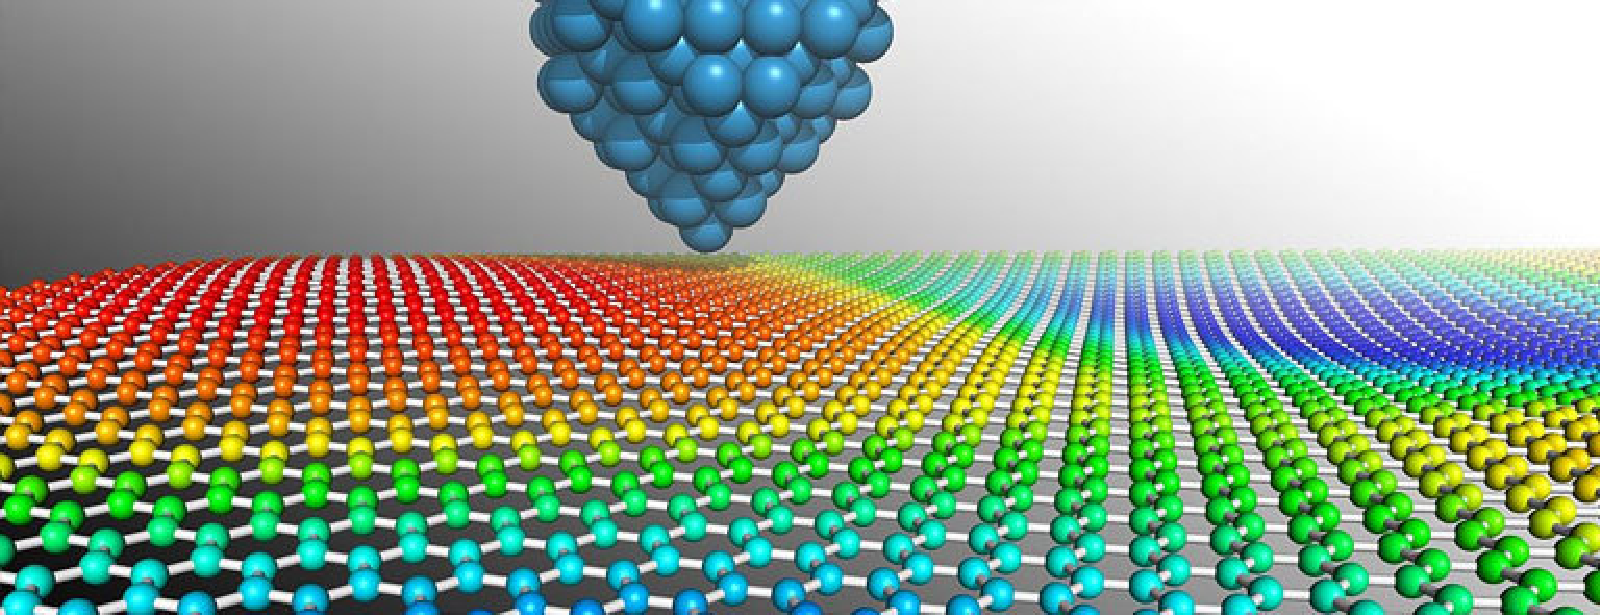
\includegraphics[width=0.25\textwidth]{out/pdf/img/material.pdf}
    {\tiny\url{http://primeurmagazine.com/flash/AE-PF-09-15-28.html}}
  \end{itemize}
\end{frame}

%%%%%%%%%%%%%%%%% 
\begin{frame}
  \frametitle{計算が支える科学, 工学, AI, \ldots の例}
  \begin{itemize}
  \item 設計 (構造物, 剛体)

    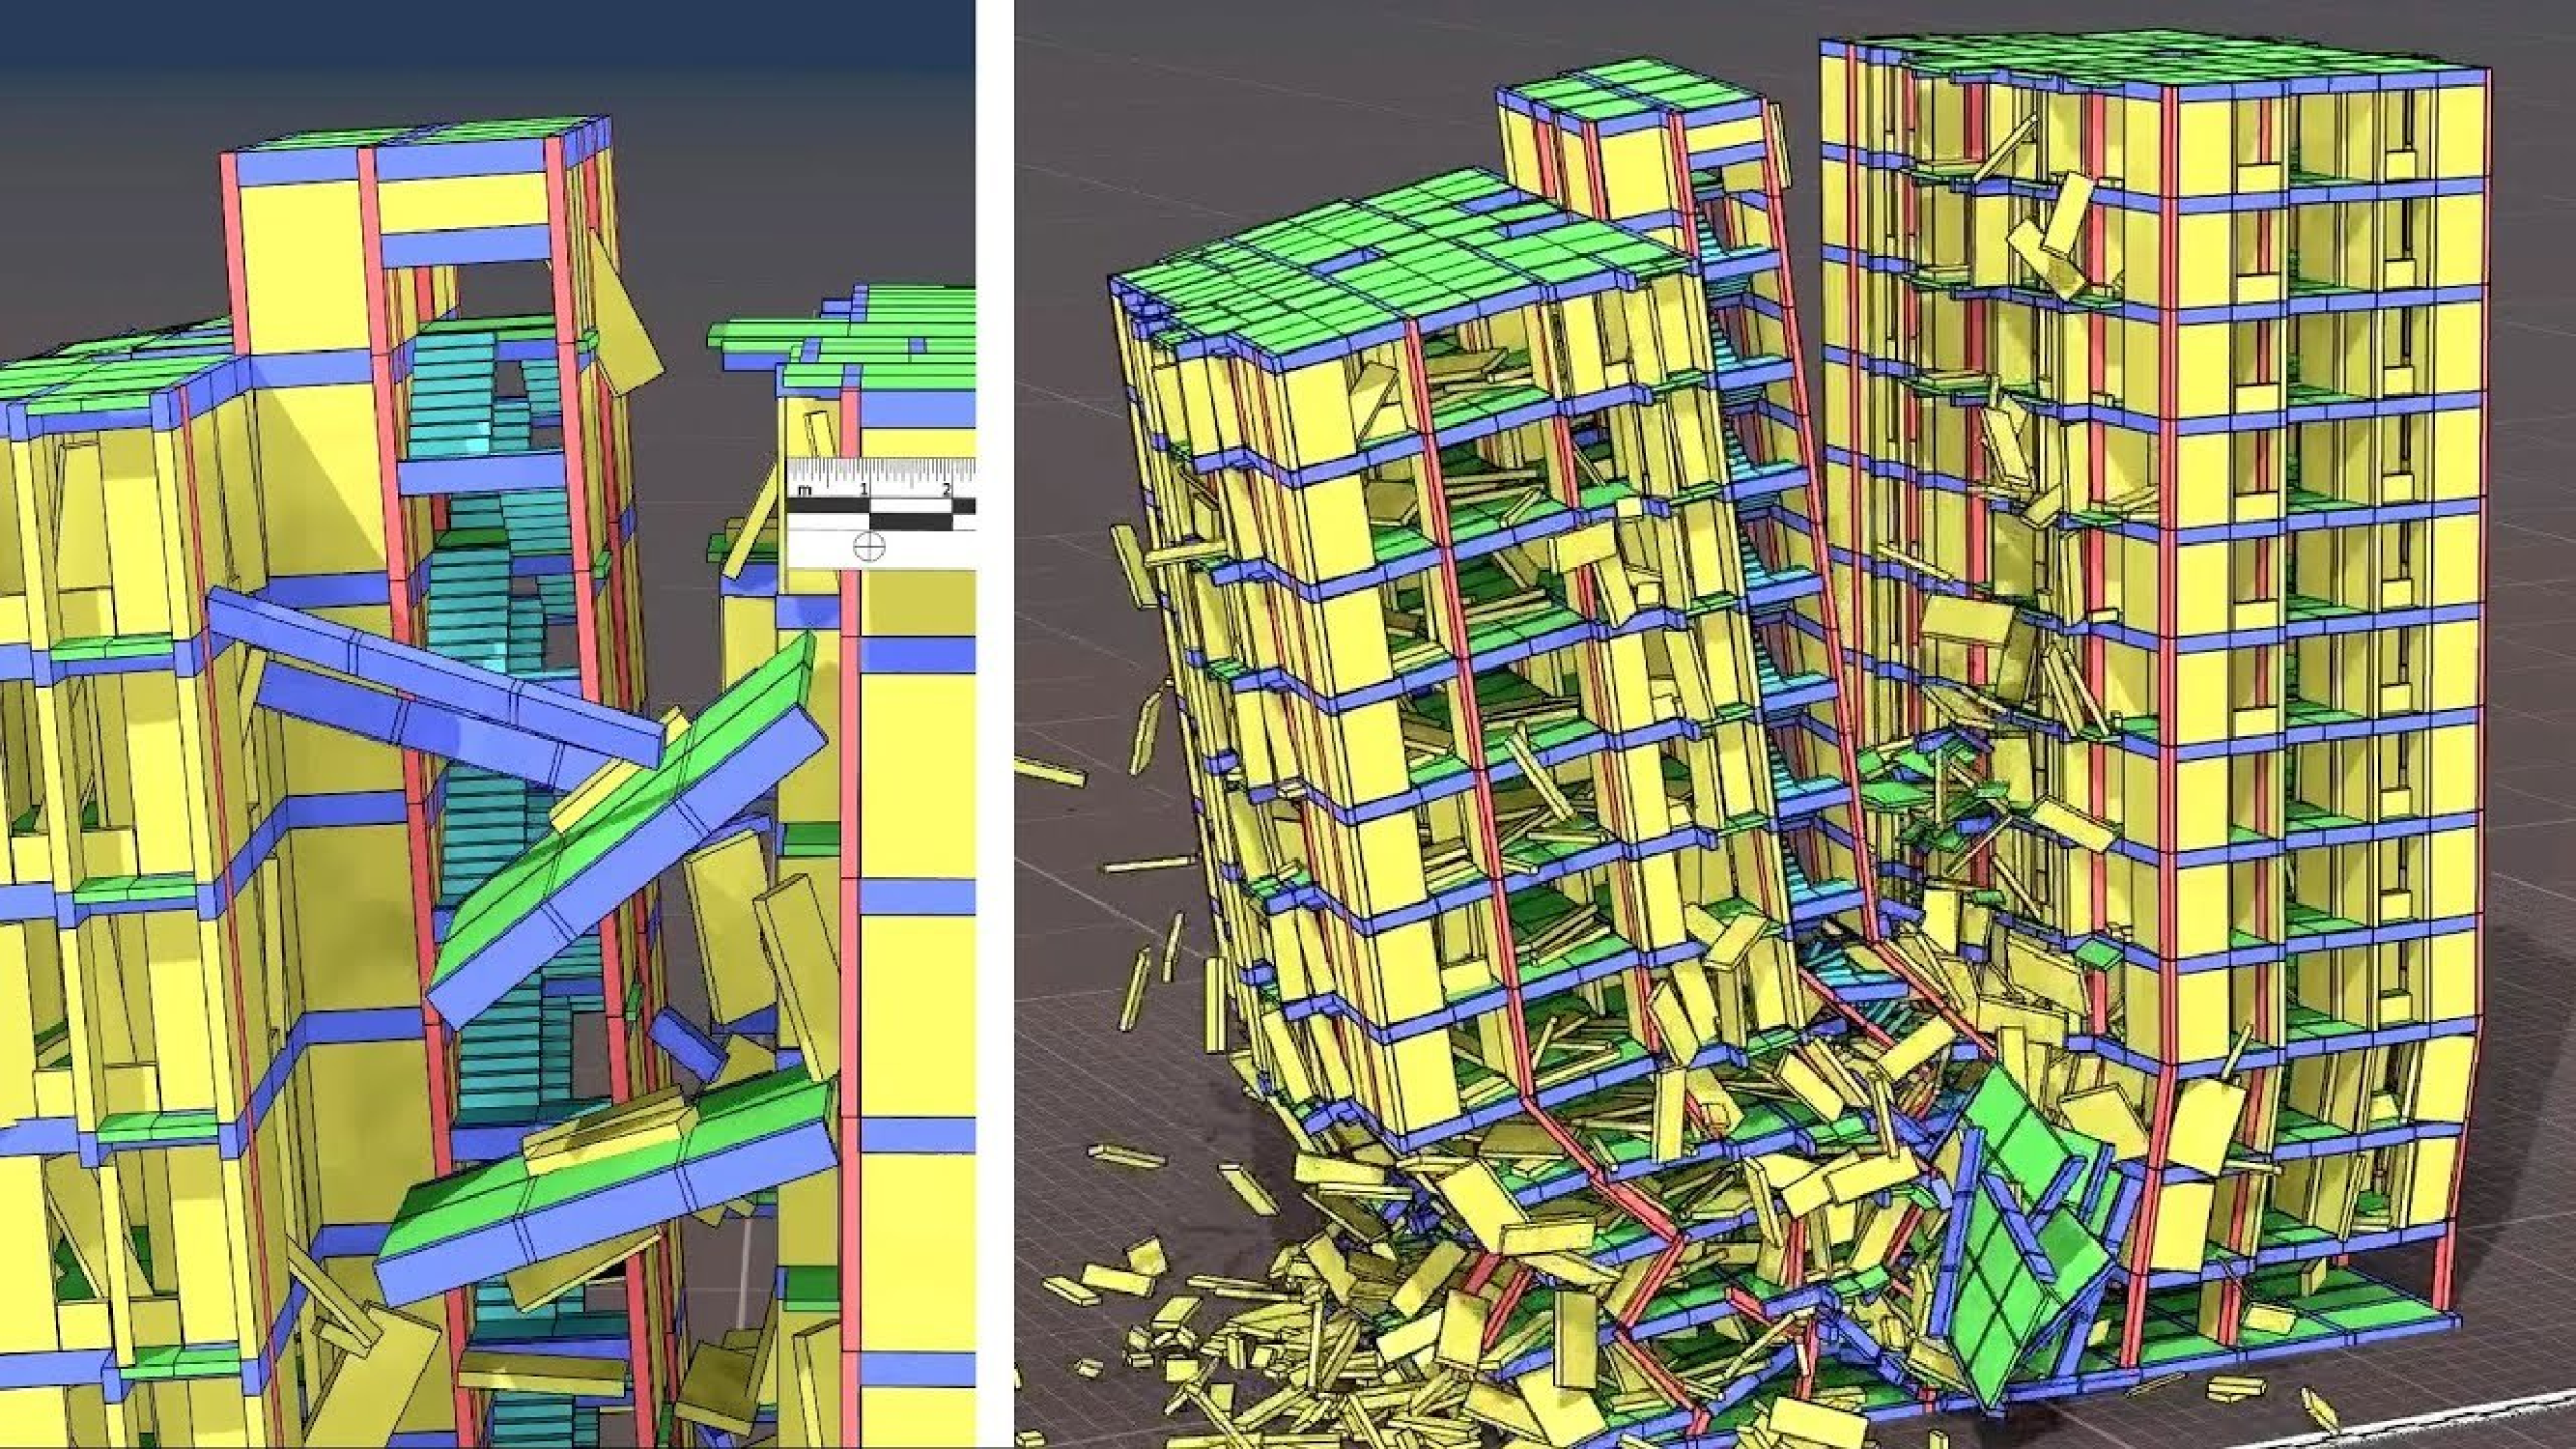
\includegraphics[width=0.25\textwidth]{out/pdf/img/building.pdf}
    {\tiny\url{https://www.youtube.com/watch?v=yu2bQtIS69g}}
  
  \item 津波 (流体)

    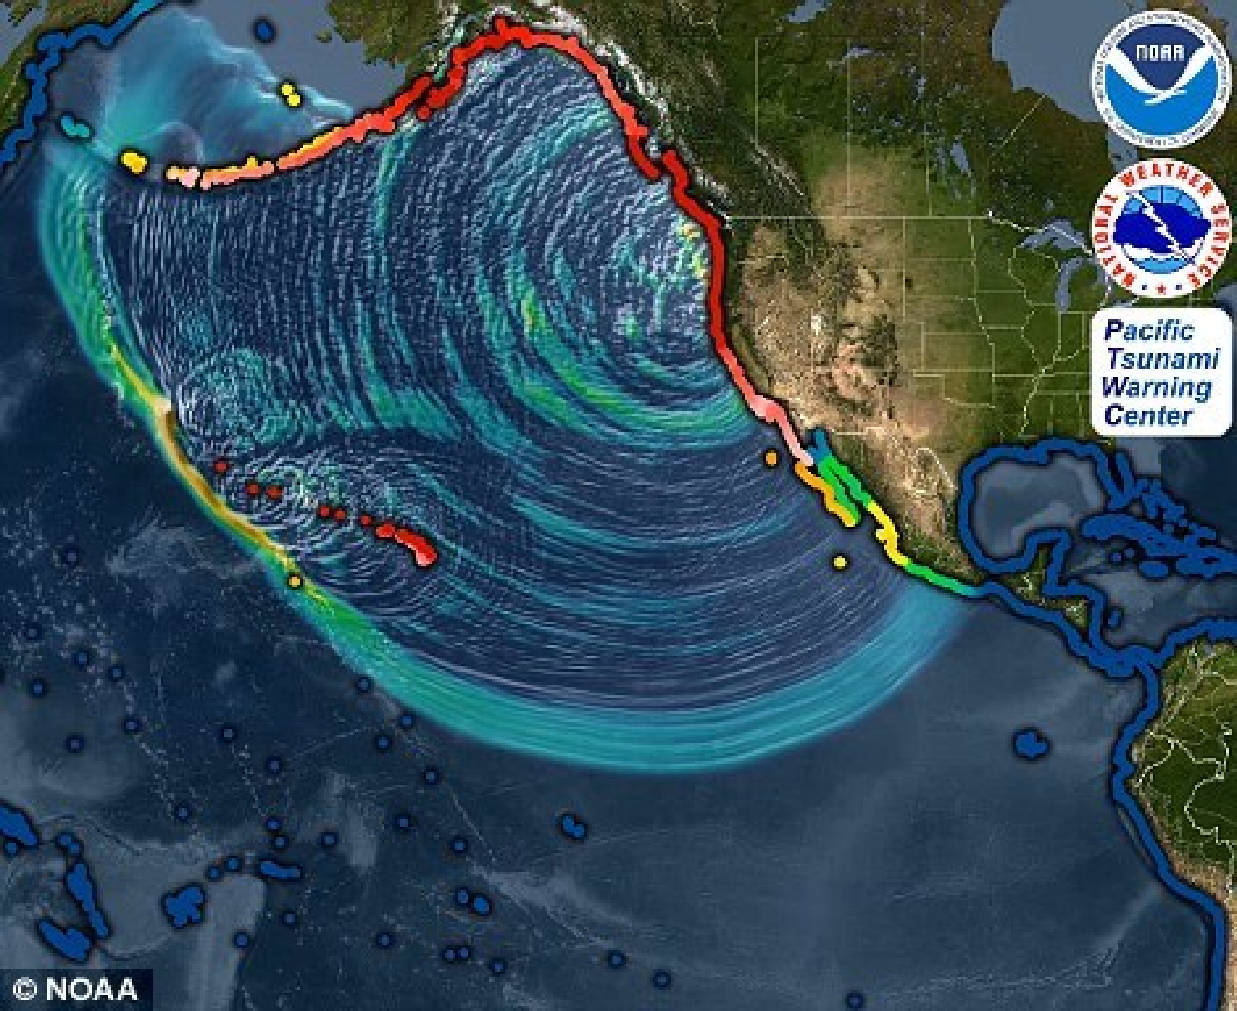
\includegraphics[width=0.25\textwidth]{out/pdf/img/tsunami.pdf}
    {\tiny\url{https://www.dailymail.co.uk/sciencetech/article-3480680/Terrifying-simulation-shows-Pacific-Northwest-decimated-megaquake-Cascadia-fault.html}}

  \end{itemize}
\end{frame}

%%%%%%%%%%%%%%%%% 
\begin{frame}
  \frametitle{計算が支える科学, 工学, AI, \ldots の例}
  \begin{itemize}
  \item 宇宙 (粒子)

    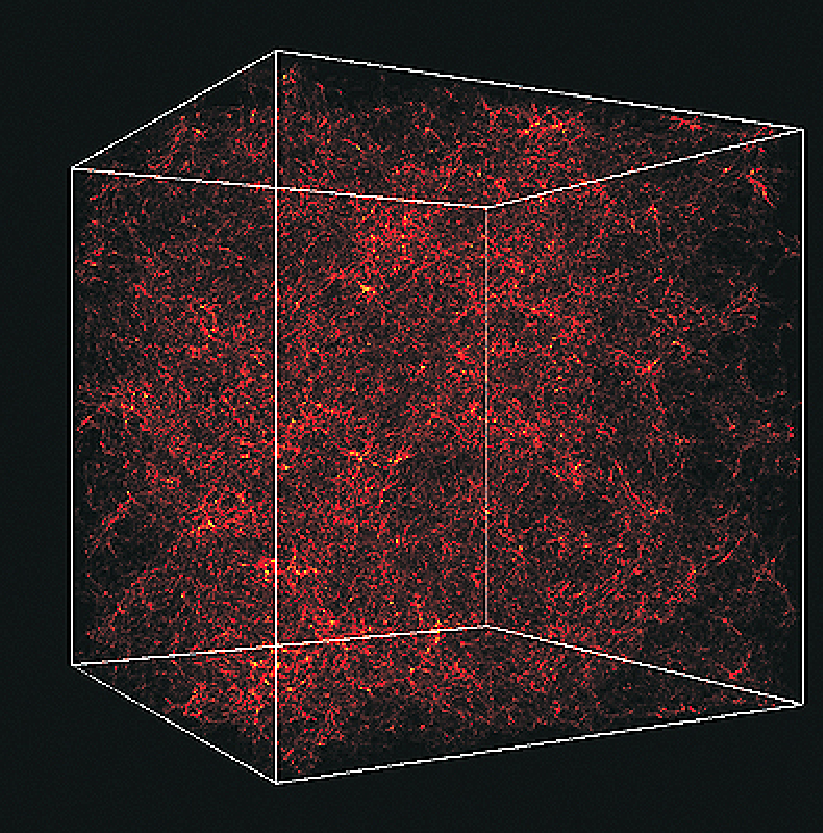
\includegraphics[width=0.25\textwidth]{out/pdf/img/darkmatter.pdf}
    {\tiny\url{http://chronicle.uchicago.edu/060713/darkmatter.shtml}}
  
  \item ゲノム・遺伝子

    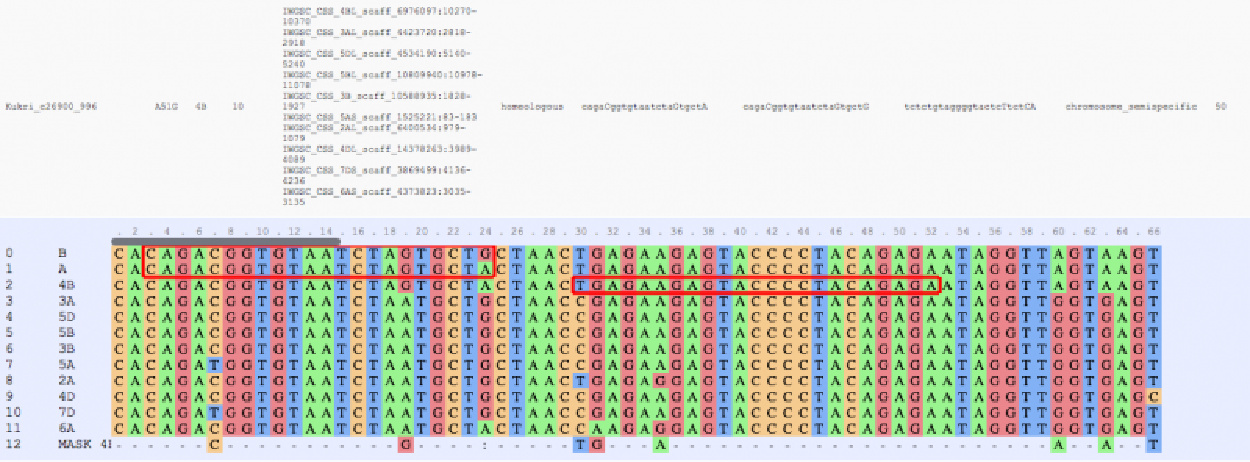
\includegraphics[width=0.25\textwidth]{out/pdf/img/genome.pdf}
    {\tiny\url{https://phys.org/news/2015-04-online-bioinformatics-tool-significantly-multiple.html}}

  \item AI

    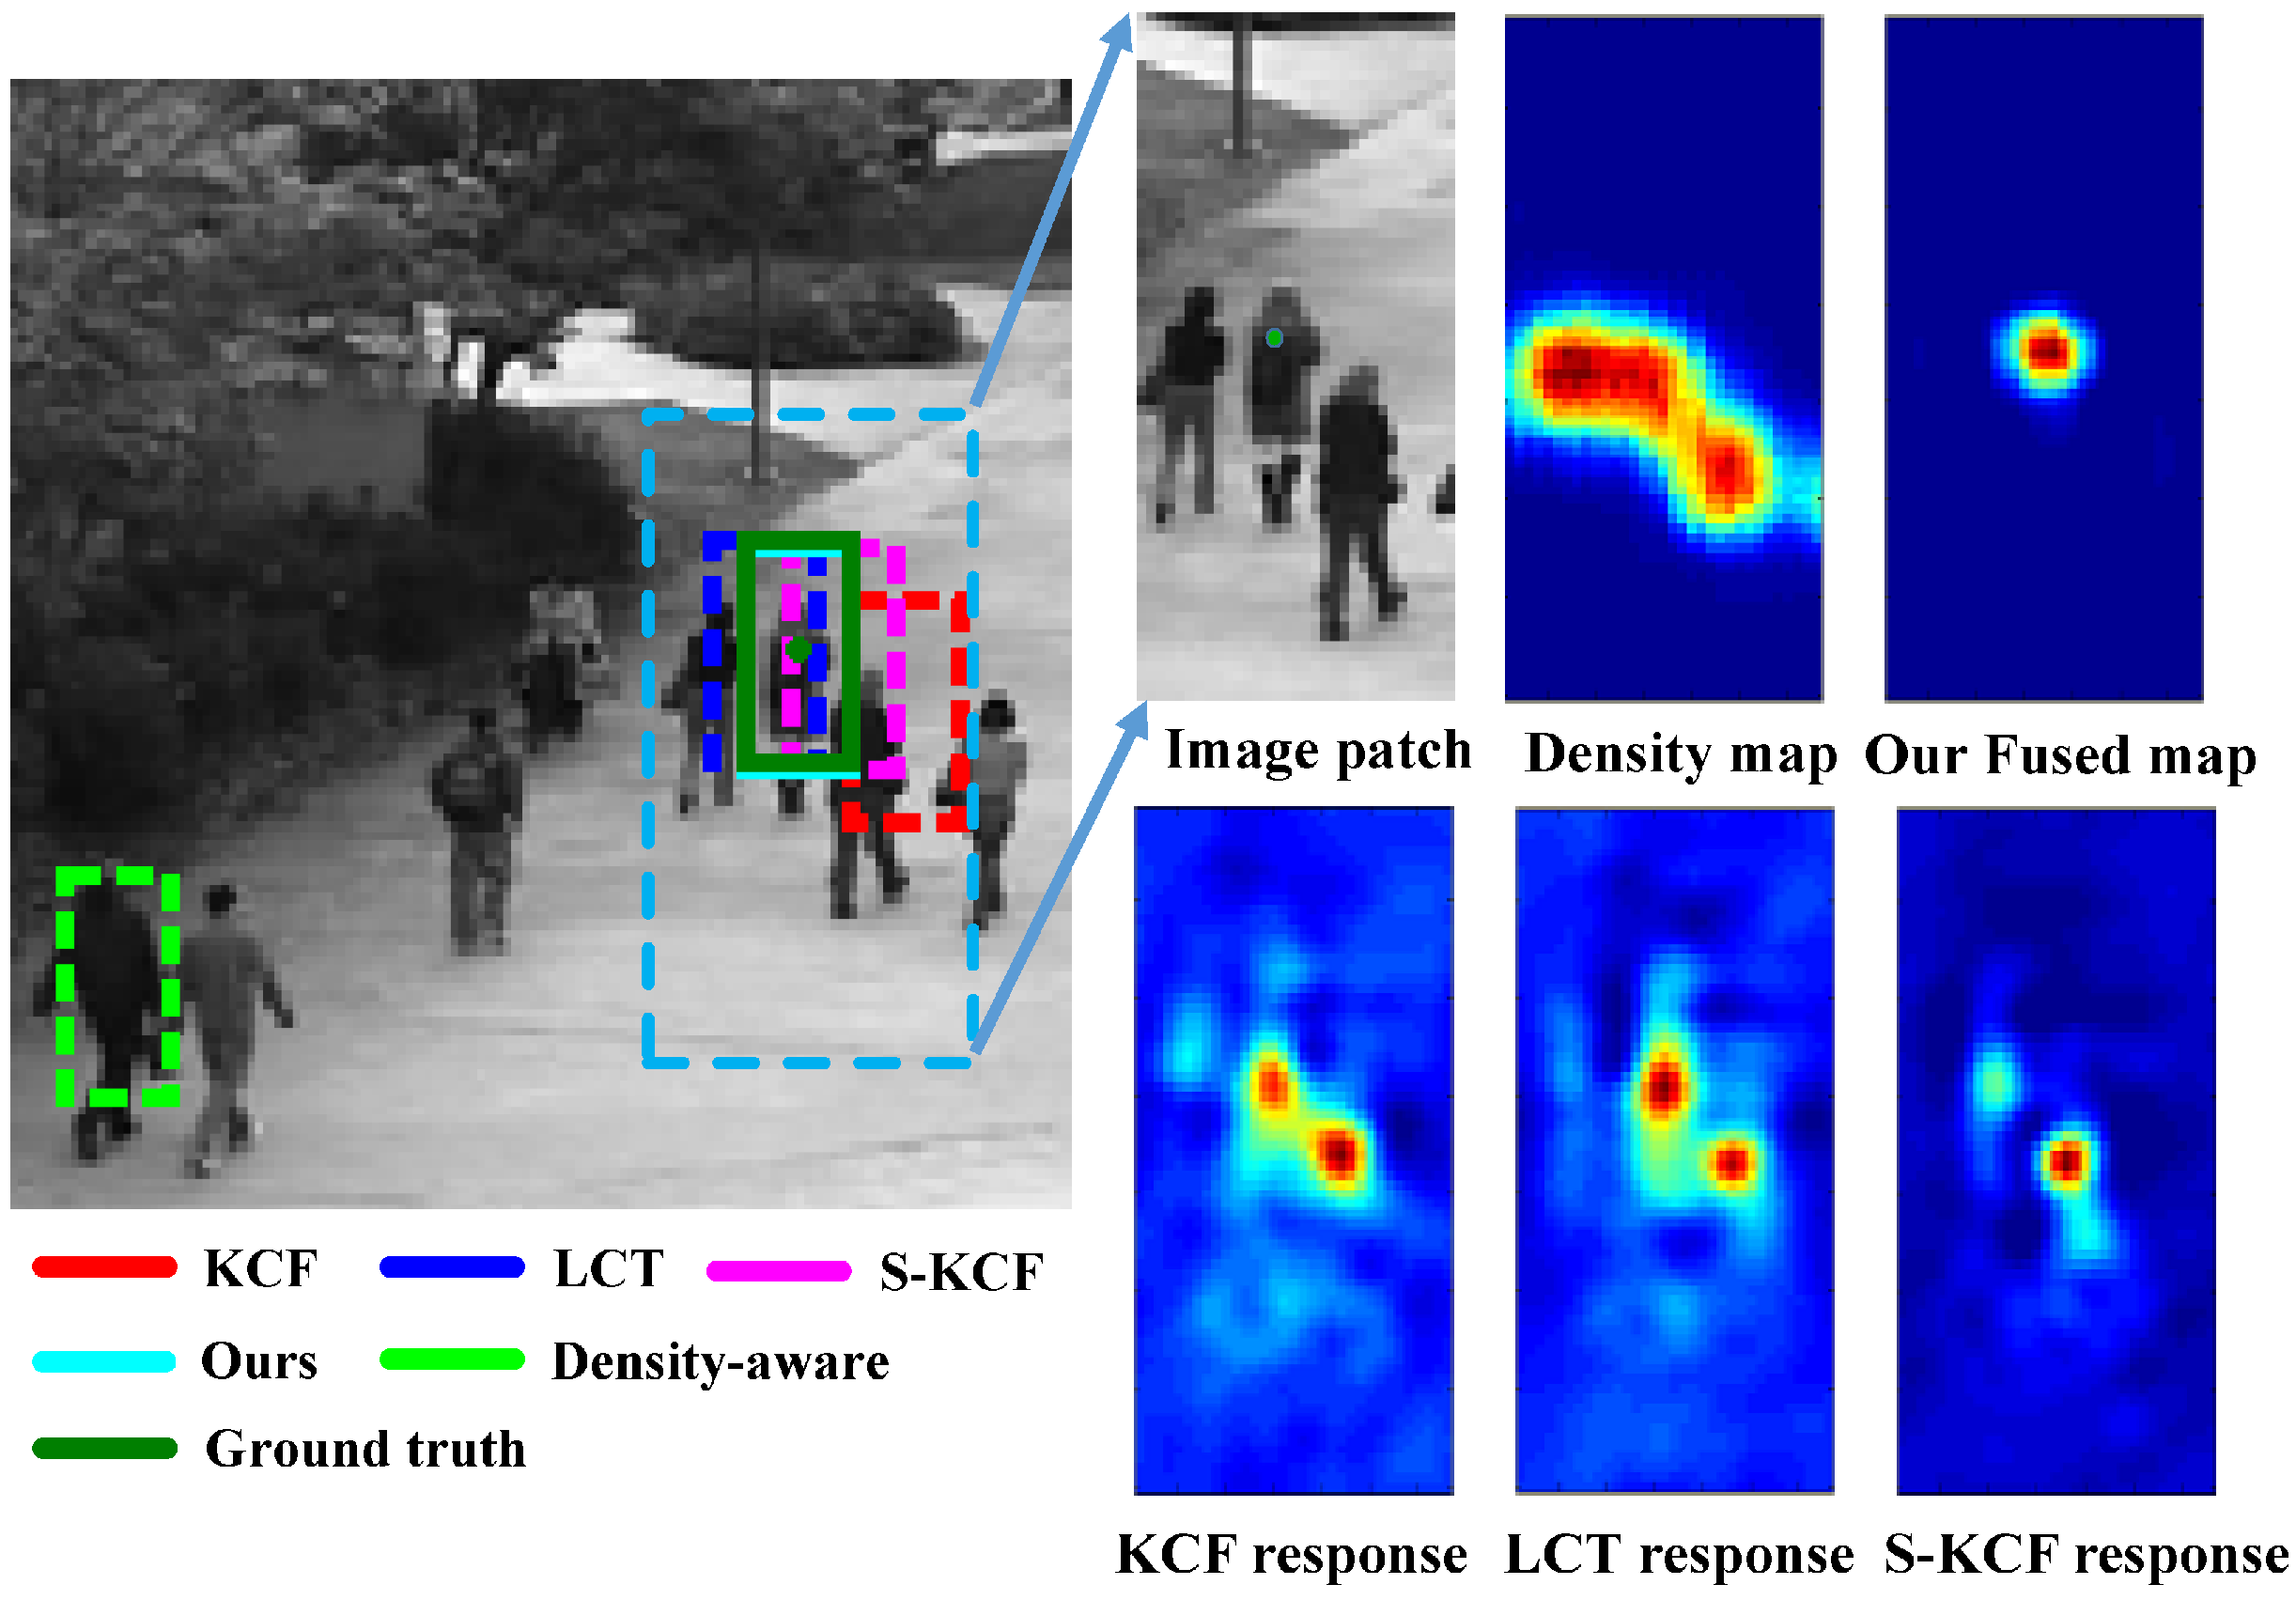
\includegraphics[width=0.25\textwidth]{out/pdf/img/ai.pdf}
    {\tiny\url{http://visal.cs.cityu.edu.hk/research/fusiont/}}
  \end{itemize}
\end{frame}

%%%%%%%%%%%%%%%%% 
\begin{frame}
\frametitle{ゼミのねらい}
\begin{itemize}
\item 実際の問題を解くことを通して,
  プログラミングを学ぶ動機を高める
\item その過程で必要な,数学・物理を知ることで,
  数学・物理を学ぶ動機を高める
\end{itemize}

% \def\svgwidth{0.4\textwidth}
% \input{out/tex/svg/math_phys_prog.pdf_tex}

\begin{figure}[htbp]
  \centering
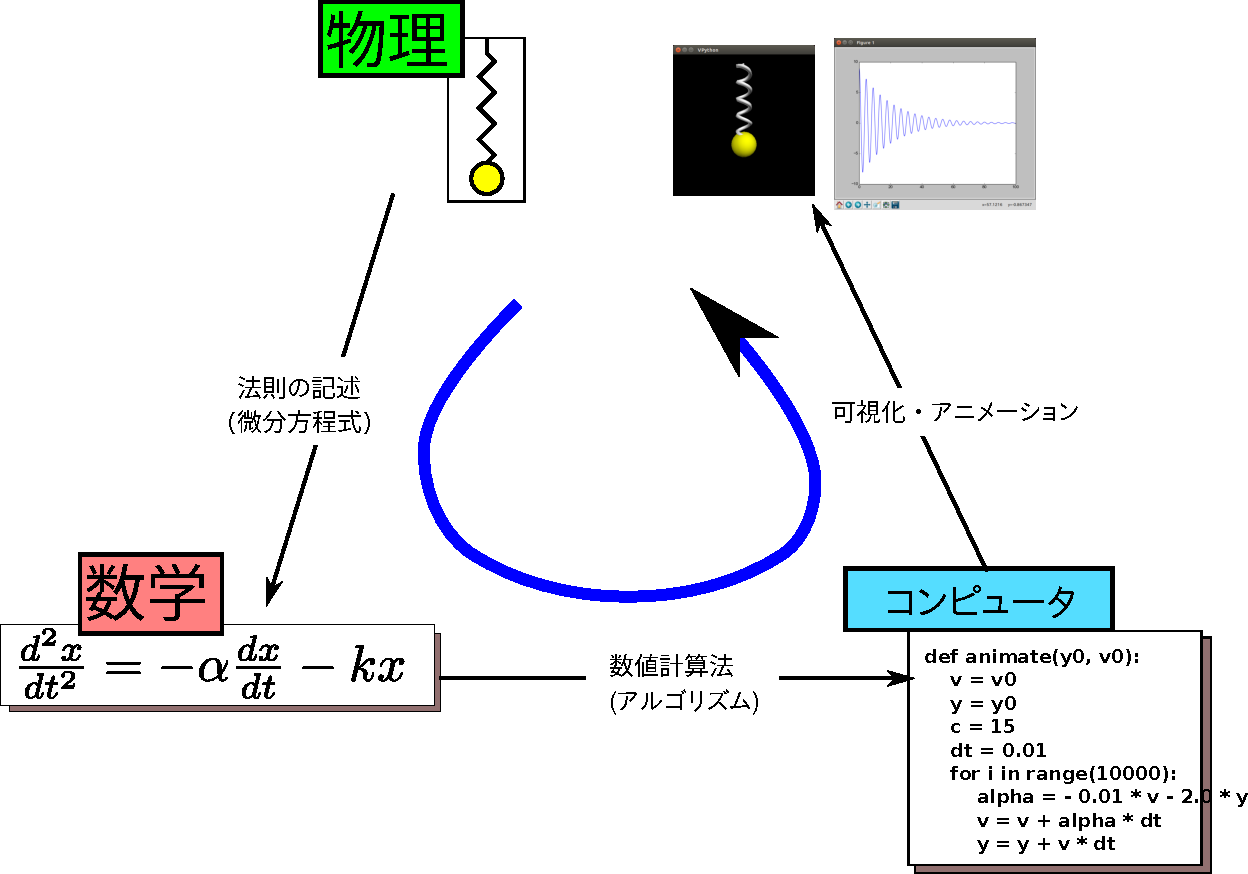
\includegraphics[width=0.7\textwidth]{out/pdf/svg/math_phys_prog_3.pdf}
\end{figure}

\end{frame}

%%%%%%%%%%%%%%%%% 
\begin{frame}
\frametitle{ゼミのロードマップ}
\begin{enumerate}
\item コンピュータで問題を解くって?
\item 道具(Python プログラミング言語)の紹介
\item 道具の練習
\item チームの結成 (3人一組)
\item 問題を解く,発展させる by チーム
\item 発表
\end{enumerate}
\end{frame}

%%%%%%%%%%%%%%%%% 
\begin{frame}

コンピュータで問題を解くって?

\end{frame}


%%%%%%%%%%%%%%%%% 
\begin{frame}
\frametitle{コンピュータにやらせやすい計算}
\begin{itemize}
\item 具体的な数値を用いた,近似的な計算
\item 記号的な計算(人間が普段やっている多くの計算)
はやらせにくい(「難しいプログラミングが必要」)
\end{itemize}
\end{frame}


%%%%%%%%%%%%%%%%% 
\begin{frame}
\frametitle{例: 微分}
\[ f(x) = x^2 \mbox{の微分} \]
\begin{itemize}
\item (記号微分) $f'(x) = 2x$ $\Rightarrow$ 難しい
\item (数値的な微分) $f'(3) \approx 6$ $\Rightarrow$ 易しい
\[ f'(3) \approx \frac{f(3+0.0001) - f(3)}{0.0001} = 6.0001 \]
\end{itemize}

$g(x) = e^{\sin x^{\sin x}} + \frac{\arcsin x}{x^3 - x^2 + 4x + 8}$
でも,数値的な微分なら同じくらい易しい
\end{frame}

%%%%%%%%%%%%%%%%% 
\begin{frame}
\frametitle{例: 積分}
\[ \int_2^3 \log x \, dx \]

\begin{itemize}
\item (記号積分) 
\[ \int_2^3 \log x \, dx = \left[ x \log x - x \right]_2^3 = \ldots \]
$\Rightarrow$ 難しい

\item (数値積分) $x_i = 2 + i/100000$ として,
\[ \int_2^3 \log x \, dx \approx  \sum_{i=0}^{99999} \log x_i \, (x_{i+1}-x_i) \]
$\Rightarrow$ 易しい
\end{itemize}
\end{frame}


%%%%%%%%%%%%%%%%% 
\begin{frame}[fragile]
\frametitle{例: 運動方程式}
空気抵抗$+$バネの力の運動方程式:

\[ \ddot{x(t)} = - \dot{x}(t) - x(t) \]

\begin{itemize}
\item (記号積分) 
\[ x(t) = \ldots \mbox{ なんだったっけ \ldots } \]

\item (数値積分) 

\begin{lstlisting}
x = 初期状態の位置;
v = 初期状態の速度;
以下を繰り返す {
  加速度 = - v - x;
  v = v + 加速度 @$\times$@ 0.001;
  x = x + v @$\times$@ 0.001;
}
\end{lstlisting}
\end{itemize}

これが「常微分方程式を解く」基本

\end{frame}

%%%%%%%%%%%%%%%%% 
\begin{frame}[fragile]
\frametitle{例: ○○方程式}
\begin{itemize}
\item 現実に求めたいものの多くは「場所と時間の関数」
\item 例: 温度の分布, 電場, 磁場, 流速の分布, 圧力の分布, 電子の密度, \ldots
\item $T(x, t)$の「一瞬あとの値」$T(x, t+\Delta t)$は, 
  $T(x, t)$や, そのまわりの値$T(x\pm \Delta x, t)$など
  から影響を受ける
\item これが「偏微分方程式」
\item コンピュータで解く場合は, たくさんの変数の「一瞬後の値」を計算していく
\item 「定常状態(変化のなくなった状態)」を求める場合, 
  巨大な連立一次方程式がでてくる
\end{itemize}
\end{frame}

%%%%%%%%%%%%%%%%% 
\begin{frame}[fragile]
\frametitle{例: 確率}
あるテニスの対戦では,各ポイントで,
プレイヤーA, Bがポイントを取る確率がそれぞれ0.52, 0.48である.
Aが1ゲーム(4ポイント先取,3-3になったら2ポイント差がつくまで)
とる確率は? 

\begin{itemize}
\item 乱数という便利な道具
\item 1ゲームのシミュレーション:
\begin{lstlisting}
a = 0
b = 0
ゲームの決着がつくまで以下を繰り返す {
  if (乱数が0.52以下) a = a + 1
  else b = b + 1
}
\end{lstlisting}
\item これを何度も何度も繰り返して,
Aがゲームを取る確率を求める
\end{itemize}
\end{frame}

%%%%%%%%%%%%%%%%% 
\begin{frame}
\frametitle{頭の使いどころ}

\begin{itemize}
\item 計算に誤差がつきまとう
  \begin{itemize}
  \item 最悪の場合,定性的に全く違う答えを出してしまうこともある
  \item 原理的にそれが回避できないような系(カオス)もある
  \end{itemize}
\item いくらコンピュータが速くても,
  たちまち計算時間が膨大になる
  \begin{itemize}
  \item 1次元の積分 100000 等分 ?
  \item 2次元の積分 100000 $\times$ 100000等分 ?
  \item 3次元の積分 \ldots 
  \end{itemize}
\end{itemize}

同じ誤差で,より計算量の少ない計算法を考えるのは,
知的・チャレンジング・
\aka{数学や物理を学ぶ意欲を高める{\tiny (と僕は思う)}}

\end{frame}

\end{document}


%%%%%%%%%%%%%%%%% 
\begin{frame}

去年の問題を少し紹介

\begin{itemize}
\item 今年版に鋭意更新中
\end{itemize}

\end{frame}

\iffalse
%%%%%%%%%%%%%%%%% 
\begin{frame}
\frametitle{問題1 最大最小}
\begin{itemize}
\item 空中で正四面体を様々な向きに配置する.
\item 正四面体の真上から,平行光線で影を作る.
\item 影の面積の最大,最小を求めよ.
\end{itemize}
\end{frame}
\fi


%%%%%%%%%%%%%%%%% 
\begin{frame}
\frametitle{問題1 ゲームの確率}

ブラックジャックの,
「ヒット・ステイ」の正解を求める
(すでにめくれているカードを考慮しない場合とする場合)

\begin{figure}[htbp]
  \centering
  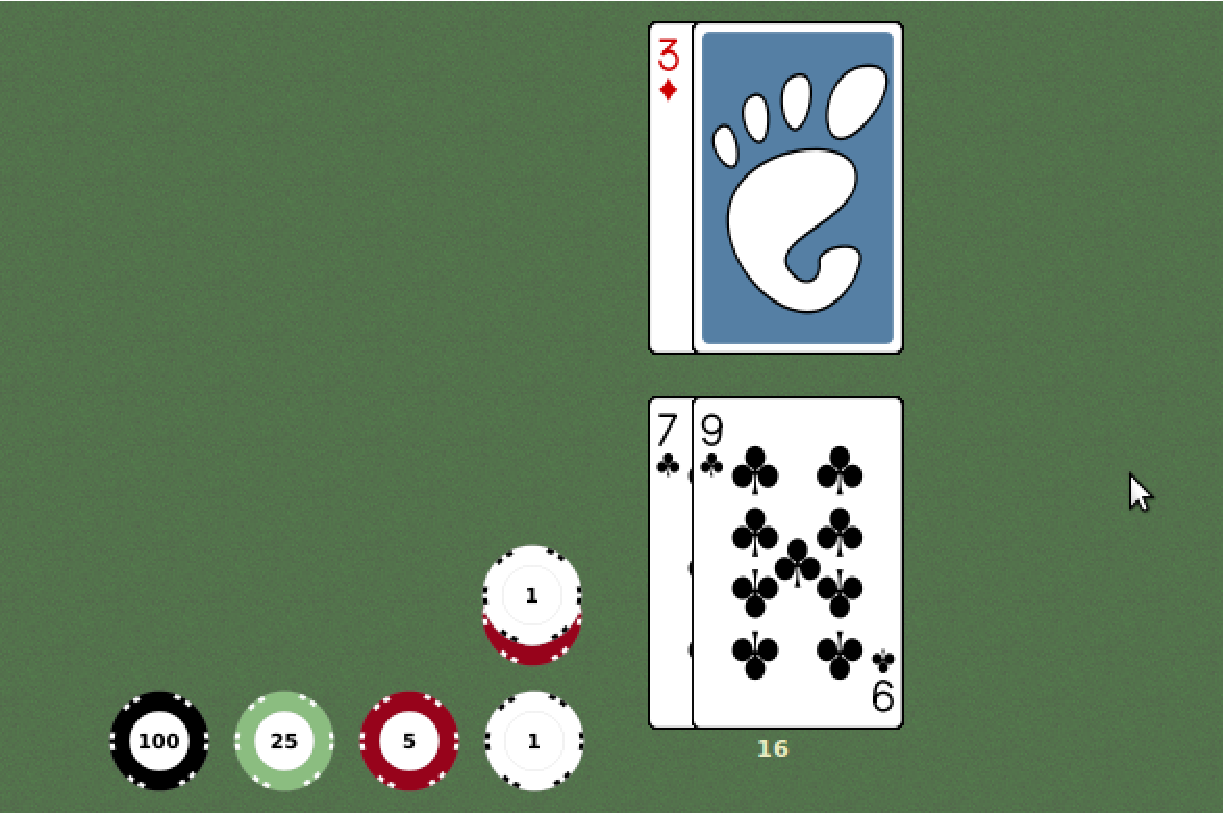
\includegraphics[width=0.5\textwidth]{blackjack.pdf}
\end{figure}

\end{frame}


%%%%%%%%%%%%%%%%% 
% 問題
% 実際の空気抵抗の測定
% 噴出される水量および速度の式は?
\begin{frame}
\frametitle{問題2 飛行距離}

\begin{columns}[t]
\begin{column}{0.7\textwidth}
\begin{wideitemize}
	\item ペットボトルロケットを遠くまで飛ばしたい
	\begin{wideitemize2}
		\item 容量$V$、重さ$M$のペットボトルロケットに、水を$V_{water}$入れる
		\item 空き容量$V-V_{water}$に、ボトルの耐圧の限界$P$まで空気を入れる
		\item 傾ける角度$\theta$を決めて、打ち出す
		\item 空気抵抗は速度に比例し、その係数を$k$とする
		\item 最適な$V_{water}$、$\theta$はいくつだろう?
	\end{wideitemize2}
	\item ちなみに、
	\begin{wideitemize2}
		\item 単純な斜方投射は角度45度で飛距離最大
		\item 実際のペットボトルロケットでは、50~60度で飛ばす指示が多い
	\end{wideitemize2}

\end{wideitemize}

\end{column}
\begin{column}{0.3\textwidth}
\begin{figure}[htbp]
    \centering
    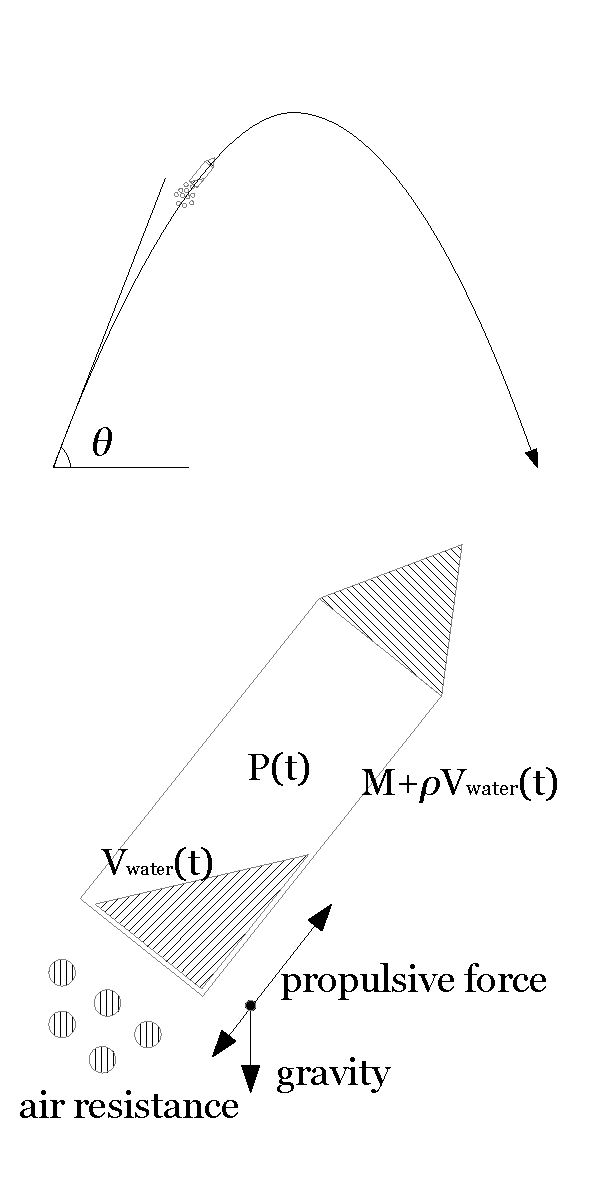
\includegraphics[bb=0mm 0mm 100.0mm 170.0mm, scale=0.35, type=pdf]{problem1.pdf}
	% http://atsites.jp/yoshitoharada/1150_Water-rocket1.jpg
\end{figure}
\end{column}
\end{columns}
\end{frame}


%%%%%%%%%%%%%%%%%%%%%%%%%%%%%%%%%%%%%%%%%%%%%%%%%%%%%%%%%%%%%%%%%%%%%%%%%%%%%%%%%%%%%%%%%%%%%%%%%%%%%%%%%%%%

% 問題
% 「地震に耐える」の定義
% バネ定数の合計が「最小」あるいは「最大」、どちらを求めるべきか(バネが柔らかいと弱い建物になりそうなため、「最小」でいいのかな?)
% 「同じエネルギーを持つ地震」は表現として不適切だが、振動数と振幅の関係を長々と書いてもなぁという印象
% モデルが正しいのか不明。各階層は床で、柱で上下を支えるモデルもあるらしい
\iffalse
\begin{frame}
\frametitle{問題3 耐震}
\begin{columns}[t]
\begin{column}{0.7\textwidth}
\begin{wideitemize}
	\item 低コストで、一定の大きさの地震に耐えられる構造物を作りたい
	\begin{wideitemize2}
		\item $L \times M \times N$個のグリッド(質量$m_{l,m,n}$)が格子状に結ばれる構造物を想定
		\item 格子部分は、バネ定数$k_{(l,m,n)\to(l',m',n')}$の建築資材で構成
		\item 同じエネルギーを持つ、振動数が$f_{min}$から$f_{max}$の地震に耐えなければならない
		\item バネ定数の合計$\sum k$が最小となる$k$は各々どのように与えればいいだろう?
	\end{wideitemize2}
	\item ちなみに、
	\begin{wideitemize2}
		\item 一般に建築物は固有振動数を持ち、その振動数の揺れに弱い
	\end{wideitemize2}

\end{wideitemize}

\end{column}
\begin{column}{0.3\textwidth}
\begin{figure}[htbp]
    \centering
    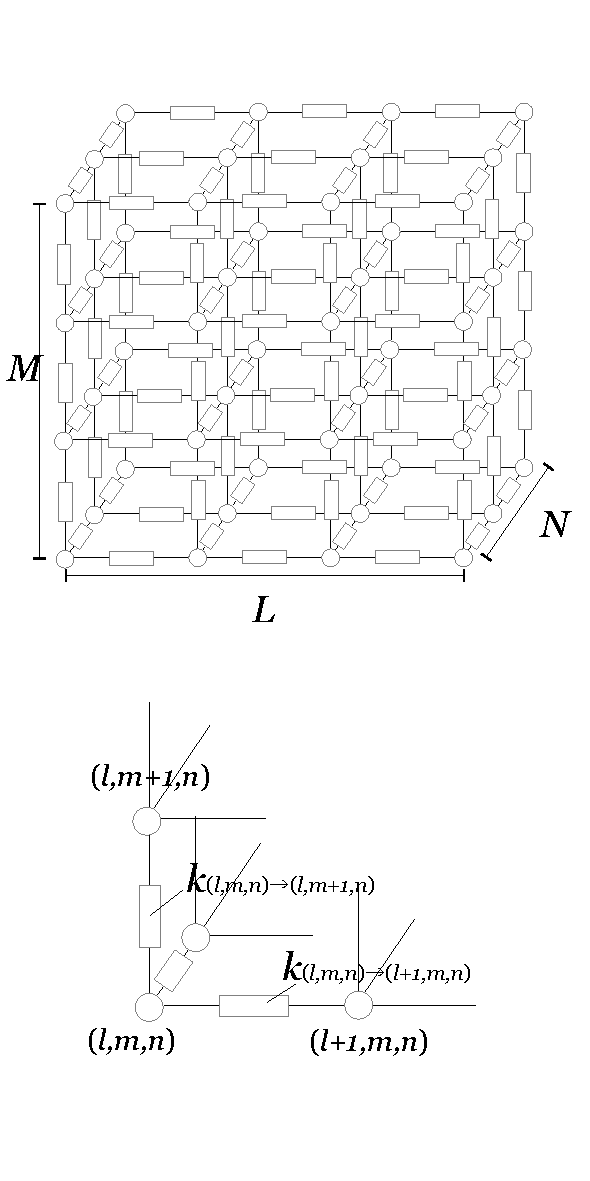
\includegraphics[bb=0mm 0mm 100.0mm 170.0mm, scale=0.35, type=pdf]{problem2.pdf}
	% http://ariel-as.eng.hokudai.ac.jp/member/image8.jpg
\end{figure}
\end{column}
\end{columns}
\end{frame}
\fi

%%%%%%%%%%%%%%%%%%%%%%%%%%%%%%%%%%%%%%%%%%%%%%%%%%%%%%%%%%%%%%%%%%%%%%%%%%%%%%%%%%%%%%%%%%%%%%%%%%%%%%%%%%%%

% 問題
% 確かめるのが難しい(理論式との比較でいいのかな?)
% 地球の自転による影響など、結構面倒くさい
% 「いつ」のパラメータが広すぎて、ヒューリスティクスを使わないと多分いい値が出ない
\begin{frame}
\frametitle{問題2 探査衛星とスイングバイ}
\begin{columns}[t]
\begin{column}{0.7\textwidth}
\begin{wideitemize}
	\item 探査機を高速にして、太陽系外に打ち出したい
	\begin{wideitemize2}
		\item 質量$m$の探査機を、地球から速度$V$、発射角度$\theta$で打ち出す
		\item プロジェクトの都合で、$N$年以内には発射しなければならない
		\item 太陽系の惑星をうまく使って、探査機の速度を最速にして打ち出したい
		\item 最適な発射角度$\theta$はいくつで、いつ打ち上げよう?
	\end{wideitemize2}
	\item ちなみに、
	\begin{wideitemize2}
		\item スイングバイは、天体の重力や運動を使い、軌道変更や加減速をすることを指す
		\item 速度が十分でないと、太陽系外に出られない
	\end{wideitemize2}

\end{wideitemize}

\end{column}
\begin{column}{0.3\textwidth}
\begin{figure}[htbp]
    \centering
    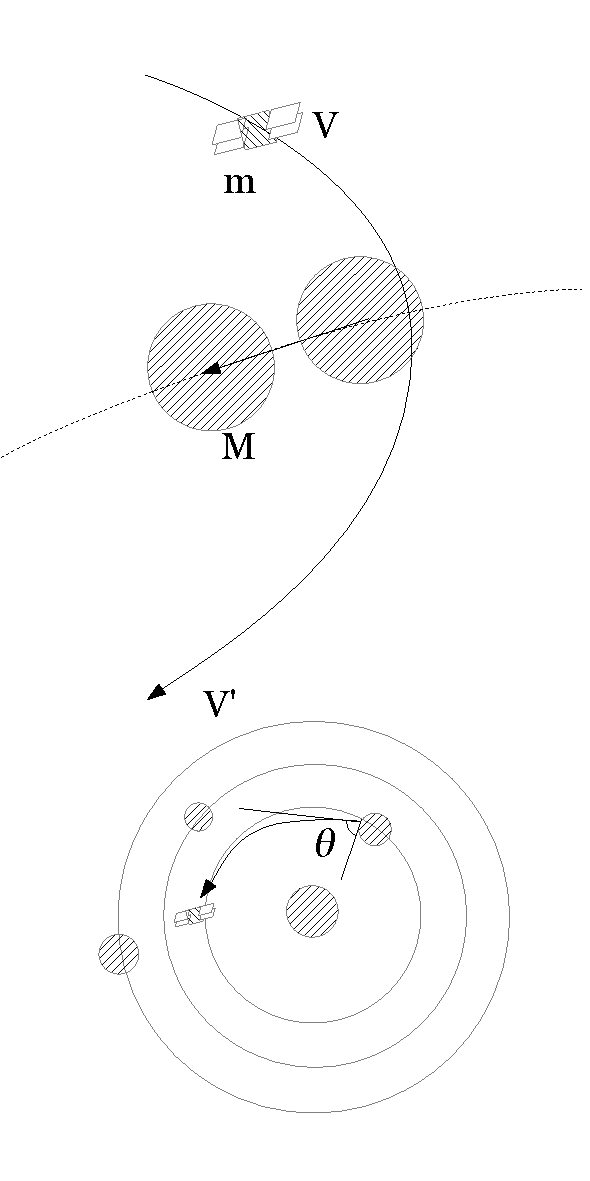
\includegraphics[bb=0mm 0mm 100.0mm 170.0mm, scale=0.35, type=pdf]{problem3.pdf}
\end{figure}
\end{column}
\end{columns}
\end{frame}

%%%%%%%%%%%%%%%%%%%%%%%%%%%%%%%%%%%%%%%%%%%%%%%%%%%%%%%%%%%%%%%%%%%%%%%%%%%%%%%%%%%%%%%%%%%%%%%%%%%%%%%%%%%%

% 問題
% 既知の音なら、行列の問題になる可能性があるという目論見
% ともかく、この問題を解くのに波動方程式を立式するのは不適当な可能性が高い
% 実用例が見つからない...。空間でやるのは実際は難しいらしい。PhasedArrayは実用化されているけど...
\begin{frame}
\frametitle{問題3 空間消音}
\begin{columns}[t]
\begin{column}{0.7\textwidth}
\begin{wideitemize}
	\item 位相を考慮した打ち消しにより、空間の騒音を低減したい
	\begin{wideitemize2}
		\item モデルとして、周期$T$の既知の音を出す騒音スピーカーが中心にある場合を考える
		\item 半径$r$の円周上に、$N$個の操作可能な消音スピーカーを用意する

		\item 円周外のある空間で、外部から受け取る音のエネルギーの総和を最小にしたい
		\item $N$個の消音スピーカーからどのような音を出せばいいだろう?
	\end{wideitemize2}
	\item ちなみに、
	\begin{wideitemize2}
		\item ノイズキャンセリングと同じ原理
		\item 一般に空間の完全消音はできない
	\end{wideitemize2}

\end{wideitemize}

\end{column}
\begin{column}{0.3\textwidth}
\begin{figure}[htbp]
    \centering
    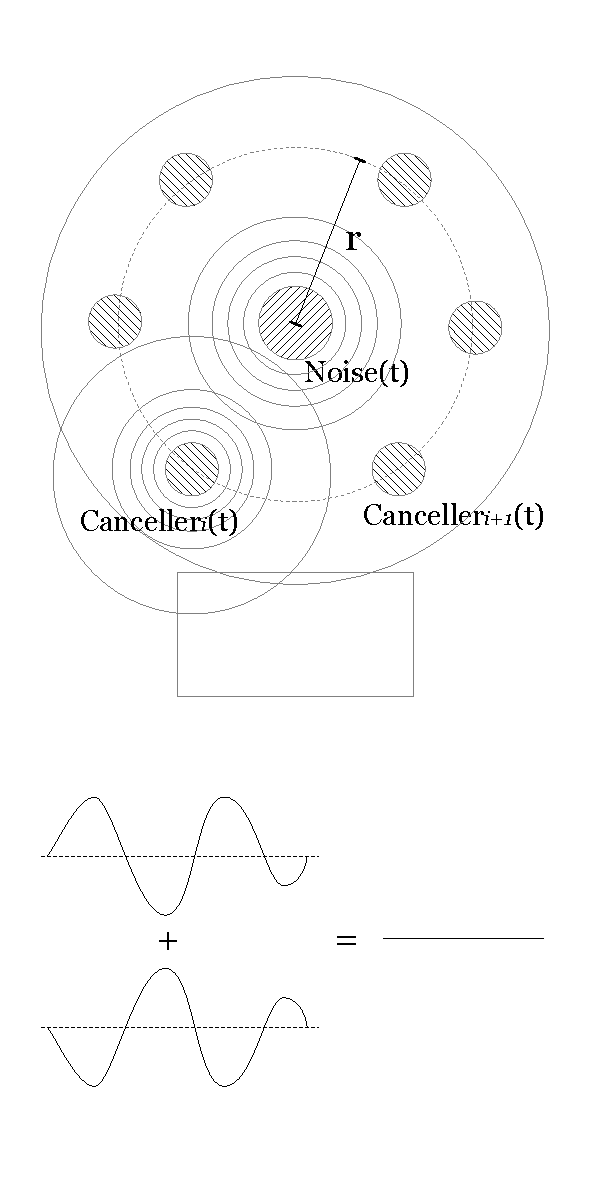
\includegraphics[bb=0mm 0mm 100.0mm 170.0mm, scale=0.35, type=pdf]{problem4.pdf}
\end{figure}
\end{column}
\end{columns}
\end{frame}

%%%%%%%%%%%%%%%%%%%%%%%%%%%%%%%%%%%%%%%%%%%%%%%%%%%%%%%%%%%%%%%%%%%%%%%%%%%%%%%%%%%%%%%%%%%%%%%%%%%%%%%%%%%%

% 問題
% 私(岩崎)は、流体系を全くやったことがないので、一から勉強しないと...
% 「形状のパラメータ化」、「ナビエ-ストークス方程式」などは与えないと無理な気もする(特に後者)
% それらしく解けるのか怪しい。メッシュで切った上での偏微分方程式のステップ計算は、pythonでちょろっと書いて計算時間が大丈夫なのか不安
% 個人的には、ボツでもいいと思っています。あるいは、後だしで「特上の難しさ」で紹介してもいいレベルです(検証が必要そう)
\begin{frame}
\frametitle{問題4 最適な翼の断面}

\begin{columns}[t]
\begin{column}{0.7\textwidth}
\begin{wideitemize}
	\item 飛行機の翼の断面を設計したい
	\begin{wideitemize2}
		\item 速度$V$で水平方向に飛ぶ飛行機を考える
		\item 内部が密で、断面積が$S$となる形状を考える
		\item 空気の流体パラメータを与える
		\item 水平方向に発生する力(抗力)$F_{drag}$を$F_{dragmax}$以下にすることを条件とする
		\item 垂直方向に発生する力(揚力)$F_{lift}$が最も大きくなる形状はなんだろう?
	\end{wideitemize2}
	\item ちなみに、
	\begin{wideitemize2}
		\item 翼の設計は、解析計算が難しい問題の典型
		\item それらしい形状が計算できたらすごい!
	\end{wideitemize2}

\end{wideitemize}

\end{column}
\begin{column}{0.3\textwidth}
\begin{figure}[htbp]
    \centering
    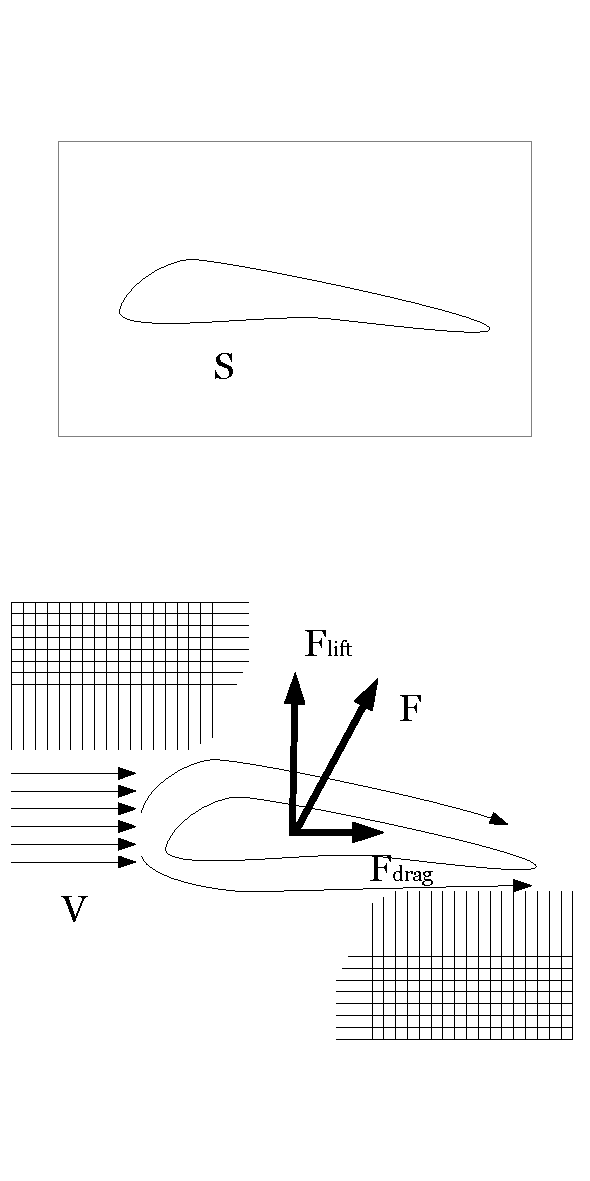
\includegraphics[bb=0mm 0mm 100.0mm 170.0mm, scale=0.35, type=pdf]{problem5.pdf}
\end{figure}
\end{column}
\end{columns}
\end{frame}

\end{document}


%%%%%%%%%%%%%%%%%%%%%%%%%%%%%%%%%%%%%%%%%%%%%%%%%%%%%%%%%%%%%%%%%%%%%%%%%%%%%%%%%%%%%%%%%%%%%%%%%%%%%%%%%%%%
% 問題
% 偉ぶっているけれども、私自身も解いたことがないので、断言できない...
% 田浦先生のスライドとかぶりそうなことを書いているので、このページは適当に削ってください
\begin{frame}{問題全体を見て}
\begin{wideitemize}
\item どれも解析的に解くのは難しいものばかり
\item 簡単そうに見えるものも、実際解こうとすると案外簡単ではない
\item 総当たりでも十分に試せるほど、パラメータ空間が狭くない
	\begin{wideitemize2}
		\item 「パラメータを0.001刻みで全部試す」のは無理なものが多い
	\end{wideitemize2}
\item 物理の知識に基づくおよその値の計算(と勘)、数学的アプローチの改良、プログラミング上の工夫などを組み合わせる必要がある
\end{wideitemize}
\end{frame}


%%%%%%%%%%%%%%%%% 
\begin{frame}
\frametitle{問題1}
(岩崎@田浦研提案と類似; $\pi$を求めて喜ぶか,体積を求めて喜ぶかかという違い)

\vskip1cm

{\LARGE 半径1の球の体積を求めよ}

\vskip2cm
{\scriptsize ひとりごと:
\begin{itemize}
\item これができれば同じ原理で,なんでもできるというのはわかるが,
  球は簡単すぎていかんせん,モチベーション的に微妙
\item 「昔苦労して計算した例」
「手計算まともにはできないが,答えがわかると嬉しい例」
とかもセットにできるとモアベター
\end{itemize}}

\end{frame}

%%%%%%%%%%%%%%%%% 
\begin{frame}
\frametitle{問題2}

{\LARGE 半径1の球の\ao{表面積}を求めよ}

\vskip2cm
{\scriptsize ひとりごと:
\begin{itemize}
\item 球面を2パラメータで表示するのが基本.
面積分の習う機会としてはよい.
\item 簡単バージョンとして「弧長を求めよ($=$ これの1次元版)」
というのもあってもいいのかも
\item パラメータ表示できない場合はどうなのという話も.
  そうでないやり方も有るのか (i.e., $f(x, y, z) = 0$ の表面積)
\item こういう,あまりにシンプルに見える問題ばかりを並べると,
数学の教科書の勉強をさせられている雰囲気が漂う危険\ldots ??
\end{itemize}}
\end{frame}


%%%%%%%%%%%%%%%%% 
\begin{frame}
\frametitle{問題4}
最大最小問題で,闇雲にはやれない(それなりに多次元)が,
最急降下とか,微分係数の方向に辿って行くとたどりつけるみたいのは,
ぜひ入れたい気が

\end{frame}



%%%%%%%%%%%%%%%%% 
\begin{frame}
\frametitle{問題5}
(安藤@田浦研君提案を単純化した)
\vskip1cm

{\LARGE
振動数既知の正弦波にノイズを載せた波を与える.
そこから元の正弦波を復元せよ.}

\vskip1.5cm

{\scriptsize ひとりごと:
\begin{itemize}
\item 実際の音声でも与えれば実用性大.
\item ただし,「正弦波」くらいからやってあげないと手も出せない可能性も大

\item 実際に音を鳴らすとなると,バイナリデータの入出力など,
  プログラミングの敷居はあがる

\item 音以外の題材で,むしろプログラミングが優しくなるようなものは?
\end{itemize}}
\end{frame}


%%%%%%%%%%%%%%%%% 
\begin{frame}
\frametitle{問題6}
ちょっと毛色の違う,今後の準備的な問題.

$n$個のお店があり,それぞれには,
そのお店の「魅力 $a_i$ (実数)」が定義されている.

ある酔っぱらいが,それらのお店をはしごする.

時刻$t$に店$i$にいた酔っぱらいは,
時刻$t+1$になるととなりの店へはしごをすることを考える.
どの店も,同じ数の「となりの店」を持つとする.

お店$j$をとなりの店の中から等確率で選び,
今のお店と魅力を比べる.

\begin{itemize}
\item $a_i \leq a_j$なら無条件で,お店$j$に移動する
\item $a_i > a_j$なら,確率$p_{ij} = a_j/a_i$で,お店$j$に移動,
確率$(1 - p_{ij})$で,お店$i$にとどまる.
\end{itemize}

十分時間立った後,酔っぱらいがお店$i$にいる確率は?

\end{frame}

%%%%%%%%%%%%%%%%% 
\begin{frame}
\frametitle{問題6 注}

\begin{itemize}
\item 答えは,$a_i / \sum_k {a_k}$, すなわち「確率が$a_i$に比例する」というわかりやすいもので,
それが実際定常状態であることもすぐにわかる.

\item そしてこれが「ある望む確率分布で乱数を発生させる」という操作に使えるという,
  有用なものだが,ちょっと唐突すぎるきらいは有る
\end{itemize}
\end{frame}



%%%%%%%%%%%%%%%%% 
\begin{frame}
\frametitle{問題7}

ややこしい確率分布に従って,平均を求めるみたいな,
単純に乱数を発生するだけでは答えが求まらないものを,
問題6を応用して求めさすみたいのを入れたい.
\end{frame}


%%%%%%%%%%%%%%%%% 
\begin{frame}
\frametitle{問題8}

最大最小問題で,問題6を利用して,関数の値が大きく(小さく)なるところで,
確率が多くなるような乱数を発生させて,
多変数の最大最小問題を解かせるみたいなのを入れたい.

\end{frame}

%%%%%%%%%%%%%%%%% 
\begin{frame}
\frametitle{問題9}
岩崎@田浦研提案

\vskip1cm

{\LARGE A から Bまでの最速降下曲線を求めよ(曲線に沿って重力のみで降下するとき,
最短時間で到達する)}

\vskip1cm

{\scriptsize ひとりごと:
\begin{itemize}
\item これが解けるなら達成度は高い
\item 解けるのかが問題.いいヒントというか,お導きが必要?
\end{itemize}}
\end{frame}


\end{document}



